% ==============================================================================
% compare_equipo_01.tex: Algorithm Comparison
% Taller 2 - Predicting Poverty | MECA 4107 | Equipo 1: Aragón, Cadena, Flórez
% Compilar desde 04_Slides con: pdflatex compare_equipo_01.tex
% ==============================================================================
\documentclass[aspectratio=169, 10pt]{beamer}
% ==============================================================================
% estilo.tex: formato común de los dos decks (best y compare)
% Taller 2 - Predicting Poverty | MECA 4107 | Equipo 1: Aragón, Cadena, Flórez
% Se compila con pdflatex. Las figuras y tablas salen de 01_Scripts/04_Results
% y 01_Scripts/02_EDA (carpeta 03_Output): ningún número se escribe a mano
% salvo los que también imprimen esos scripts.
% ==============================================================================
\usetheme[progressbar=frametitle, numbering=fraction, block=fill, sectionpage=none]{metropolis}
\usepackage[spanish, es-noshorthands]{babel}
\usepackage[utf8]{inputenc}
\usepackage[T1]{fontenc}
\usepackage[sfdefault, scaled=.92]{FiraSans}
\usepackage{booktabs, threeparttable, makecell, multirow, array, colortbl, xcolor}
\usepackage{tikz}
\usetikzlibrary{positioning, arrows.meta, shapes.geometric, fit, calc}
\graphicspath{{../03_Output/Figures/}}

% Colores (los mismos de las figuras: paleta Okabe-Ito)
\definecolor{azul}{HTML}{0072B2}
\definecolor{naranja}{HTML}{D55E00}
\definecolor{verde}{HTML}{009E73}
\definecolor{rosa}{HTML}{CC79A7}
\definecolor{gris}{HTML}{4D4D4D}
\definecolor{fondo}{HTML}{F4F6F8}
\definecolor{oscuro}{HTML}{1F2A3A}

\setbeamercolor{frametitle}{bg=oscuro, fg=white}
\setbeamercolor{progress bar}{fg=naranja, bg=oscuro!30}
\setbeamercolor{title separator}{fg=naranja}
\setbeamercolor{alerted text}{fg=naranja}
\setbeamercolor{block title}{bg=oscuro!12, fg=oscuro}
\setbeamercolor{block body}{bg=fondo}
\setbeamercolor{normal text}{fg=gris}
\setbeamerfont{frametitle}{size=\large}
\setbeamerfont{footnote}{size=\tiny}

% Tablas de kableExtra: tamaño compacto
\newcommand{\tabla}[2][\footnotesize]{{#1\renewcommand{\arraystretch}{1.15}\input{../03_Output/Tables/#2.tex}}}
% Tabla escalada a un ancho dado: \tablar{ancho}{archivo}
\newcommand{\tablar}[2]{\resizebox{#1}{!}{\input{../03_Output/Tables/#2.tex}}}
% Mensaje principal de la diapositiva (una línea, arriba)
\newcommand{\mensaje}[1]{{\color{oscuro}\bfseries #1}\par\vspace{0.4em}}
% Fuente pequeña al pie
\newcommand{\fuente}[1]{\par\vfill{\tiny\color{gris!80} #1}}
% Cifra grande
\newcommand{\cifra}[2]{\begin{tabular}[t]{@{}c@{}}{\color{naranja}\fontsize{24}{26}\selectfont\bfseries #1}\\[0.1em]\scriptsize #2\end{tabular}}

\title{Predecir la pobreza en Colombia}
\author{Equipo 1: Aragón, Cadena y Flórez}
\institute{MECA 4107 Big Data y Machine Learning para Economía Aplicada --- Universidad de los Andes}
\date{Problem Set 2 \quad\textbullet\quad Octubre de 2026}

\subtitle{Algorithm Comparison}

\begin{document}

\maketitle

% ------------------------------------------------------------------------------
% Diapositiva obligatoria: el mejor modelo (igual en los dos decks)
\begin{frame}{El mejor modelo en una diapositiva}
\mensaje{Clasificamos con un índice de ingreso construido desde las personas}
\begin{columns}[T]
\begin{column}{0.6\textwidth}
\resizebox{\linewidth}{!}{% Diagrama del mejor modelo (se usa en los dos decks)
\begin{tikzpicture}[
  font=\scriptsize, >={Stealth[length=2mm]},
  caja/.style={draw=#1, fill=#1!10, rounded corners=3pt, align=center, minimum height=8mm, inner sep=3pt, line width=0.7pt},
  caja/.default=azul, flecha/.style={->, line width=0.7pt, color=gris}]
  % Personas
  \node[caja=naranja, text width=24mm] (per) {\textbf{541 mil personas}\\variables propias\\+ de su hogar};
  \node[caja=naranja, text width=27mm, right=8mm of per, yshift=9mm] (m17) {LightGBM: ingreso total};
  \node[caja=naranja, text width=27mm, right=8mm of per] (m20) {LightGBM: + columnas\\crudas y pesos};
  \node[caja=naranja, text width=27mm, right=8mm of per, yshift=-9mm] (m22) {5 LightGBM: uno por\\componente del ingreso};
  \node[caja=naranja, text width=22mm, right=7mm of m20] (suma) {Suma por hogar\\y promedio: $\hat y$};
  \node[caja=naranja, text width=28mm, right=7mm of suma] (z) {$z = \hat y - g$\\$g$: brecha exacta del DANE\\$\sigma$: error esperado};
  \node[caja=naranja, text width=20mm, below=6mm of z] (logit) {Logit en\\$z,\ z/\sigma,\ \log\sigma$};
  % Hogar
  \node[caja=azul, text width=24mm, below=17mm of per] (hog) {\textbf{165 mil hogares}\\85 variables};
  \node[caja=azul, text width=27mm, right=8mm of hog] (xgb) {XGBoost de\\clasificación};
  % Ensamble
  \node[caja=rosa, text width=34mm, below=6mm of logit] (ens) {$P = 0.3\,P_{\text{XGB}} + 0.7\,P_{\text{ingreso}}$\\pobre si $P \geq 0.40$};
  \draw[flecha] (per.east) -- ++(3mm,0) |- (m17.west);
  \draw[flecha] (per.east) -- (m20.west);
  \draw[flecha] (per.east) -- ++(3mm,0) |- (m22.west);
  \draw[flecha] (m17.east) -- ++(3mm,0) |- (suma.west);
  \draw[flecha] (m20.east) -- (suma.west);
  \draw[flecha] (m22.east) -- ++(3mm,0) |- (suma.west);
  \draw[flecha] (suma) -- (z);
  \draw[flecha] (z) -- (logit);
  \draw[flecha] (logit) -- (ens);
  \draw[flecha] (hog) -- (xgb);
  \draw[flecha] (xgb.east) -- (xgb.east -| ens.west);
\end{tikzpicture}
}
\par\vspace{0.5em}
{\scriptsize\textbf{Especificación (boosting):} $P = 0.3\,P_{\text{XGBoost}} + 0.7\,P_{\text{ingreso}}$. El XGBoost clasifica con 85 variables del hogar. $P_{\text{ingreso}}$: tres LightGBM predicen el ingreso de cada persona; se suma por hogar, se promedian y se compara con la brecha del hogar; un logit lo convierte en probabilidad según qué tan incierta es la predicción ($\sigma$). Pobre si $P \geq 0.40$.\par}
\end{column}
\begin{column}{0.38\textwidth}
\centering
\cifra{0.77}{Kaggle público}\hspace{0.6em}\cifra{0.77}{Kaggle privado}\hspace{0.6em}\cifra{0.776}{F1 CV}
\par\vspace{0.6em}\raggedright
{\footnotesize
\begin{enumerate}\setlength\itemsep{0.25em}
\item \alert{Predecir el ingreso de cada persona} vale más que cambiar de algoritmo.
\item El desbalance se maneja con el \alert{umbral}, no rebalanceando.
\item Sin el módulo de ingresos, una encuesta corta cae a \alert{F1 0.69}.
\end{enumerate}}
\par\vspace{0.3em}
{\tiny Cuatro envíos empatan en 0.77 en el público (Kaggle muestra 2 decimales); entre ellos, el CV difiere en menos de 0.001, menos que su error estándar. Presentamos el que el equipo seleccionó.\par}
\end{column}
\end{columns}
\end{frame}


% ------------------------------------------------------------------------------
\section{Datos}

\begin{frame}{Por qué este problema premia la flexibilidad y la información}
\begin{columns}[c]
\begin{column}{0.62\textwidth}
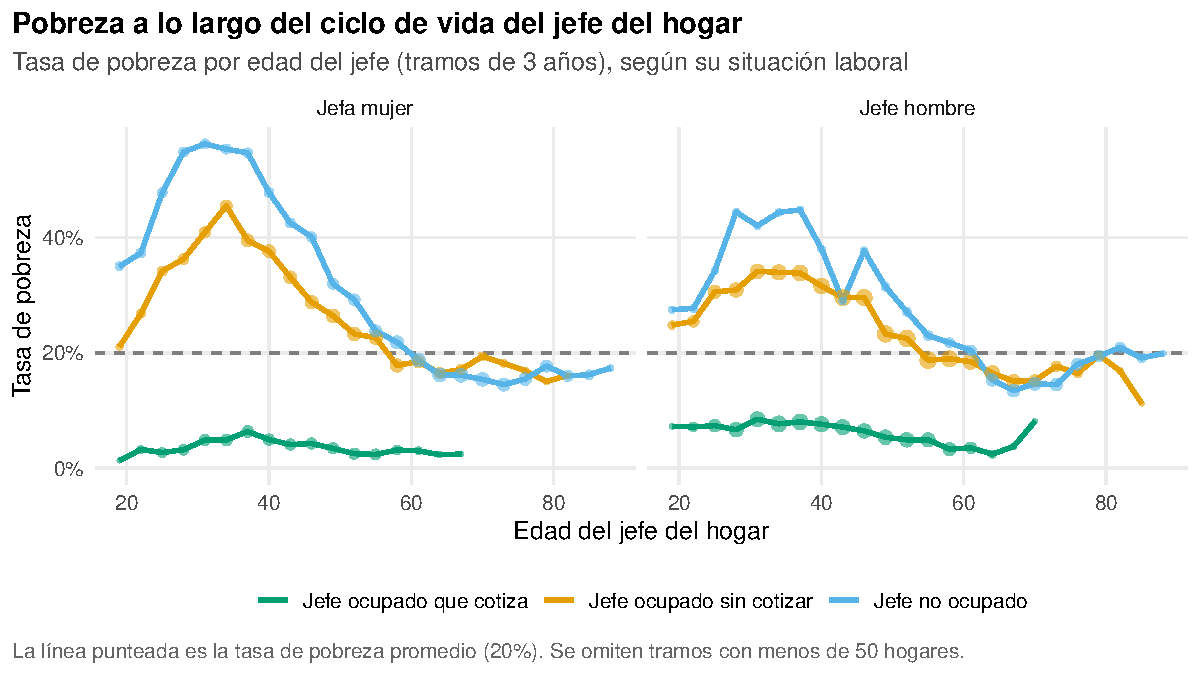
\includegraphics[width=\linewidth]{fig_ciclo_vida.pdf}
\end{column}
\begin{column}{0.37\textwidth}
\footnotesize
\begin{itemize}\setlength\itemsep{0.35em}
\item \textbf{Interacciones:} si el jefe cotiza, la pobreza es baja a cualquier edad; si no, llega a 40--55 \% entre los 30 y 40 años. Un logit necesita que le escribamos esa interacción, mientras que un árbol la encuentra solo.
\item \textbf{Umbrales:} un hogar es pobre cuando su ingreso cae por debajo de la línea, y los árboles funcionan justamente así: parten los datos con cortes.
\item \textbf{Muchos datos:} con 165 mil hogares y 85 variables, penalizar debería aportar poco.
\item \textbf{Información:} el ingreso está en las \alert{personas}, así que un modelo a nivel hogar solo ve agregados.
\end{itemize}
\end{column}
\end{columns}
\end{frame}

\begin{frame}{Un campo nivelado: la diferencia es del algoritmo}
\begin{columns}[c]
\begin{column}{0.48\textwidth}
\begin{block}{Lo mismo para todos los modelos}
\small
\begin{itemize}\setlength\itemsep{0.7em}
\item \textbf{Base:} 164,960 hogares, 85 predictores (hogar + personas agregadas), sin variables de ingreso.
\item \textbf{Validación:} los mismos 5 folds estratificados (semilla 2026).
\item \textbf{Métrica:} F1 fuera de muestra.
\item \textbf{Umbral:} el que maximiza el F1 sobre las predicciones fuera de muestra (grilla 0.01--0.99).
\item \textbf{Hiperparámetros:} búsqueda en grilla con validación cruzada.
\end{itemize}
\end{block}
\end{column}
\begin{column}{0.48\textwidth}
\begin{block}{Lo que cambia}
\small
\begin{itemize}\setlength\itemsep{0.7em}
\item \textbf{LPM y Logit:} efectos aditivos (MCO y máxima verosimilitud).
\item \textbf{Elastic Net:} logit con penalización $L_1 + L_2$.
\item \textbf{CART:} un árbol podado por $cp$.
\item \textbf{Random Forest:} promedio de 300 árboles profundos, cada uno con una muestra distinta de hogares y de variables.
\item \textbf{Boosting:} árboles poco profundos en secuencia, cada uno corrige al anterior.
\end{itemize}
\end{block}
\end{column}
\end{columns}
\end{frame}

% ------------------------------------------------------------------------------
\section{Comparación de algoritmos}

\begin{frame}{Los seis algoritmos: boosting gana con las mismas variables}
\centering
\tablar{0.95\linewidth}{tab_algoritmos}
\par\vspace{0.6em}
{\small Los dos más cercanos al boosting en Kaggle son \alert{Random Forest} y \alert{Logit} (0.73 público; 0.741 y 0.739 en CV).}
\end{frame}

\begin{frame}{Un solo árbol encuentra las variables correctas, pero en escalones}
\begin{columns}[c]
\begin{column}{0.71\textwidth}
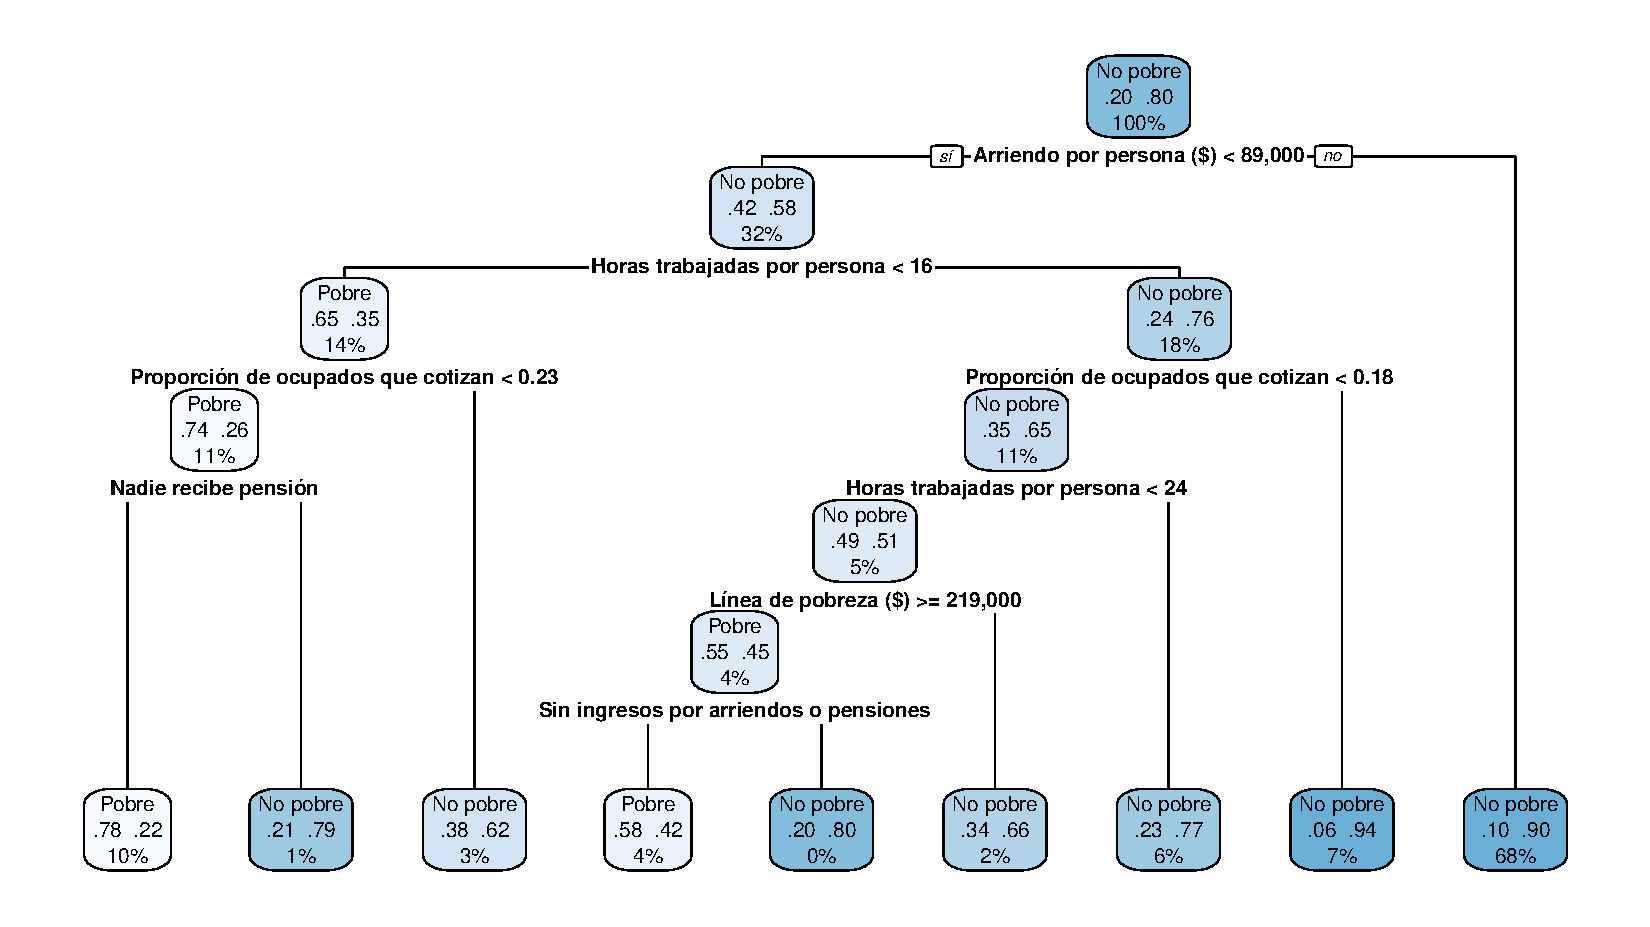
\includegraphics[width=\linewidth]{fig_arbol.pdf}
\end{column}
\begin{column}{0.28\textwidth}
\footnotesize
Los primeros cortes son los de la teoría: \alert{arriendo por persona}, \alert{horas trabajadas}, ocupados que \alert{cotizan} y pensiones.
\par\vspace{0.8em}
\renewcommand{\arraystretch}{1.2}
\scriptsize\begin{tabular}{@{}l>{\raggedright\arraybackslash}p{1.75cm}r@{}}
\toprule
& Qué hace & F1 \\
\midrule
CART & Un árbol: escalones & 0.704\\
Logit & Suma efectos & 0.739\\
RF & Promedia árboles: menos varianza & 0.741\\
XGBoost & Suma árboles: menos sesgo & 0.760\\
\bottomrule
\end{tabular}
\end{column}
\end{columns}
\end{frame}

\begin{frame}{Búsqueda de hiperparámetros: afinar mueve poco el F1}
\begin{columns}[c]
\begin{column}{0.7\textwidth}
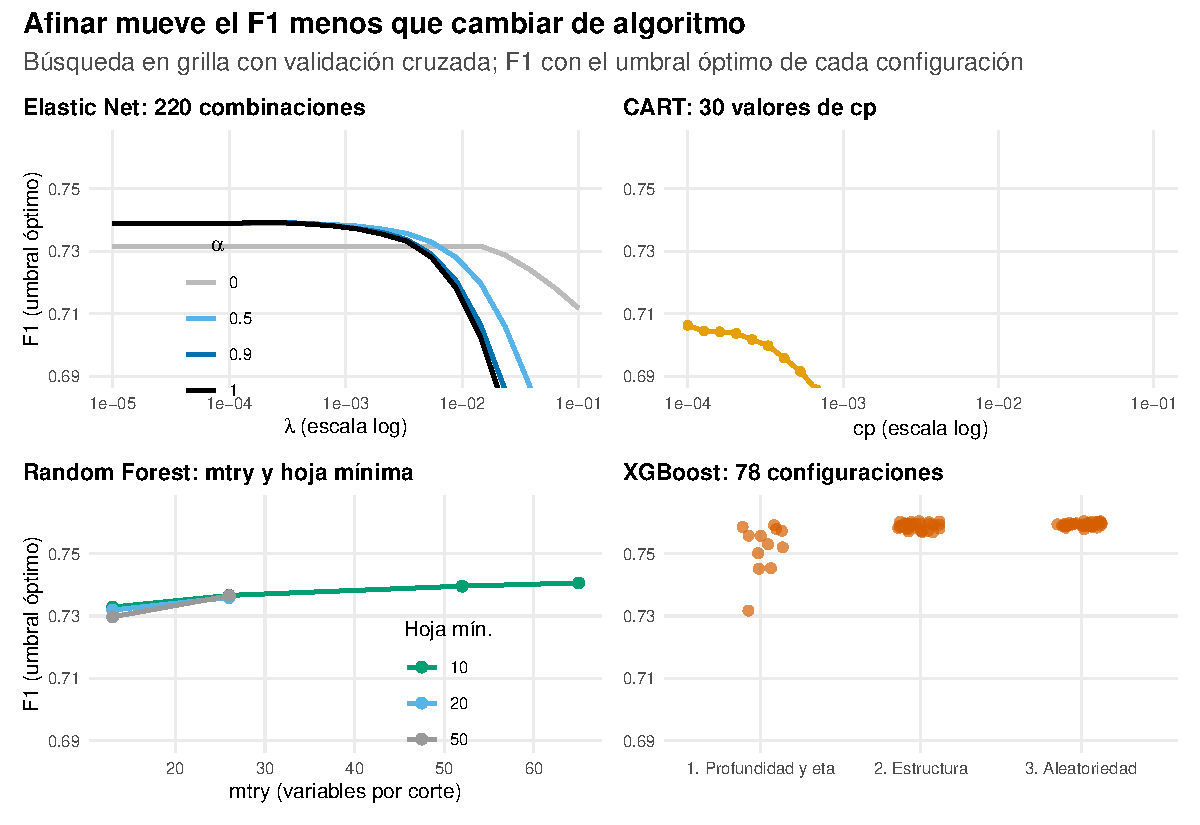
\includegraphics[width=\linewidth]{fig_tuning.pdf}
\end{column}
\begin{column}{0.29\textwidth}
\footnotesize
\begin{itemize}
\item \textbf{Elastic Net:} el óptimo es casi sin penalización ($\lambda \approx 0.0003$): regularizar no ayuda con 165 mil hogares.
\item \textbf{RF:} lo que importa es cuántas \alert{variables candidatas} ve cada corte (13 a 65); árboles profundos.
\item \textbf{XGBoost:} 78 configuraciones entre 0.757 y 0.760: una meseta.
\end{itemize}
\end{column}
\end{columns}
\end{frame}

\begin{frame}{Boosting frente a Random Forest y Logit, en igualdad de condiciones}
\centering
\tablar{0.8\linewidth}{tab_campo_nivelado}
\par\vspace{0.8em}\raggedright
\begin{columns}[T]
\begin{column}{0.32\textwidth}
\begin{block}{Logit (0.739)}
\small Efectos aditivos. Las interacciones económicas hechas a mano sumaron solo 0.001.
\end{block}
\end{column}
\begin{column}{0.32\textwidth}
\begin{block}{Random Forest (0.741)}
\small Capta interacciones, pero promediar árboles profundos reduce \alert{varianza}, no sesgo. Lo que más pesa es cuántas variables ve cada corte.
\end{block}
\end{column}
\begin{column}{0.32\textwidth}
\begin{block}{Boosting (0.760)}
\small Cada árbol corrige el error del anterior: reduce \alert{sesgo}. Ventaja de +0.02, entre 10 y 15 veces su error estándar.
\end{block}
\end{column}
\end{columns}
\end{frame}

\begin{frame}{Dónde gana el boosting: en todos los grupos, sobre todo en hogares pequeños}
\centering
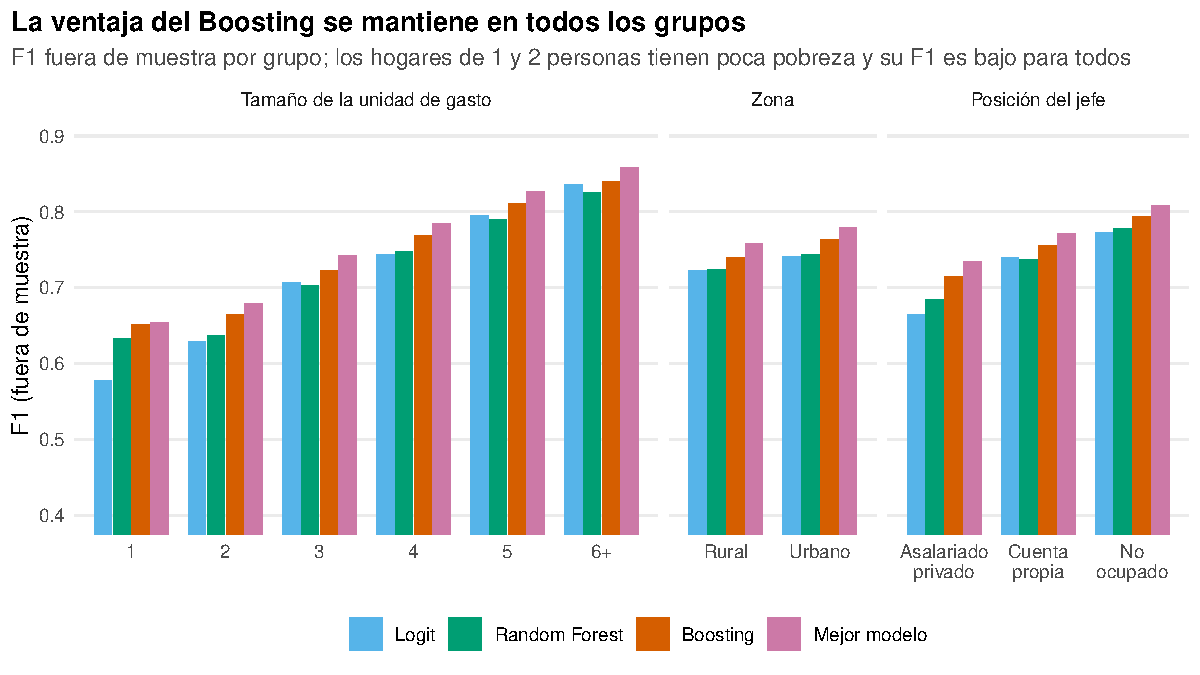
\includegraphics[height=0.84\textheight]{fig_f1_grupos.pdf}
\end{frame}

\begin{frame}{Dónde fallan todos: cerca de la línea de pobreza}
\begin{columns}[c]
\begin{column}{0.73\textwidth}
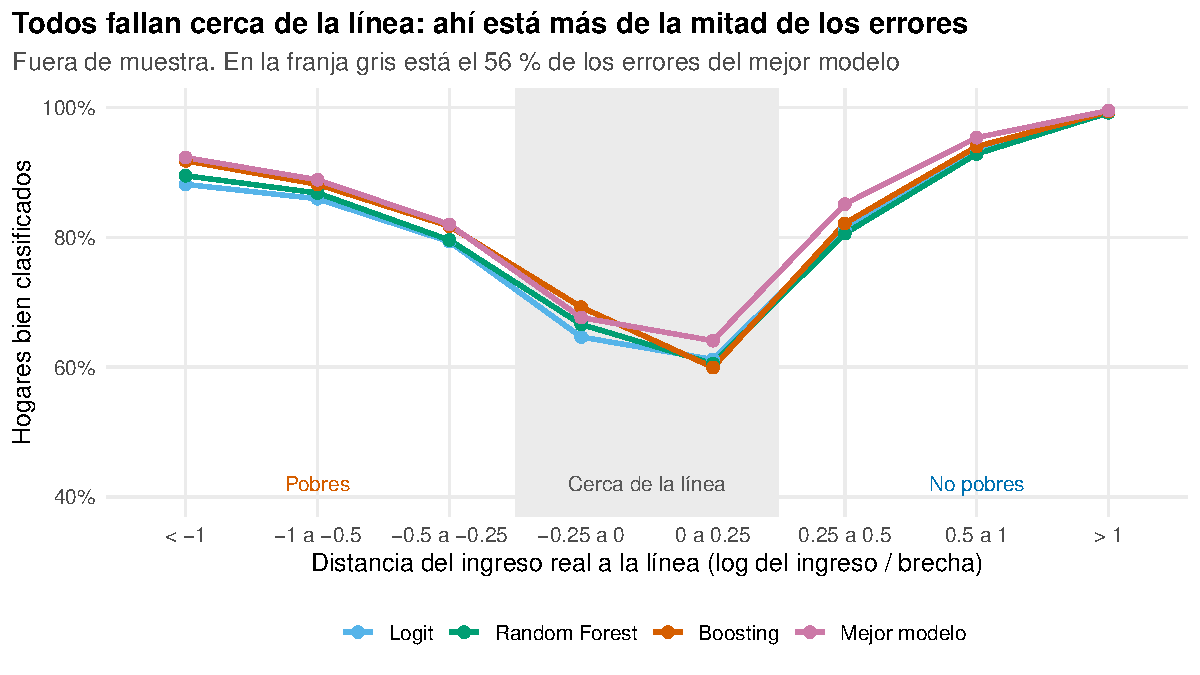
\includegraphics[width=\linewidth]{fig_distancia_linea.pdf}
\end{column}
\begin{column}{0.26\textwidth}
\footnotesize
\begin{itemize}
\item Lejos de la línea, todos aciertan más del 90 \%.
\item Cerca de la línea ($\pm 0.25$ log) aciertan 60--70 \%: ahí está más de la mitad de los errores.
\item Ningún algoritmo arregla eso; solo \alert{más información} sobre el ingreso.
\end{itemize}
\end{column}
\end{columns}
\end{frame}

\begin{frame}{El desbalance: tres estrategias, el umbral gana}
\centering
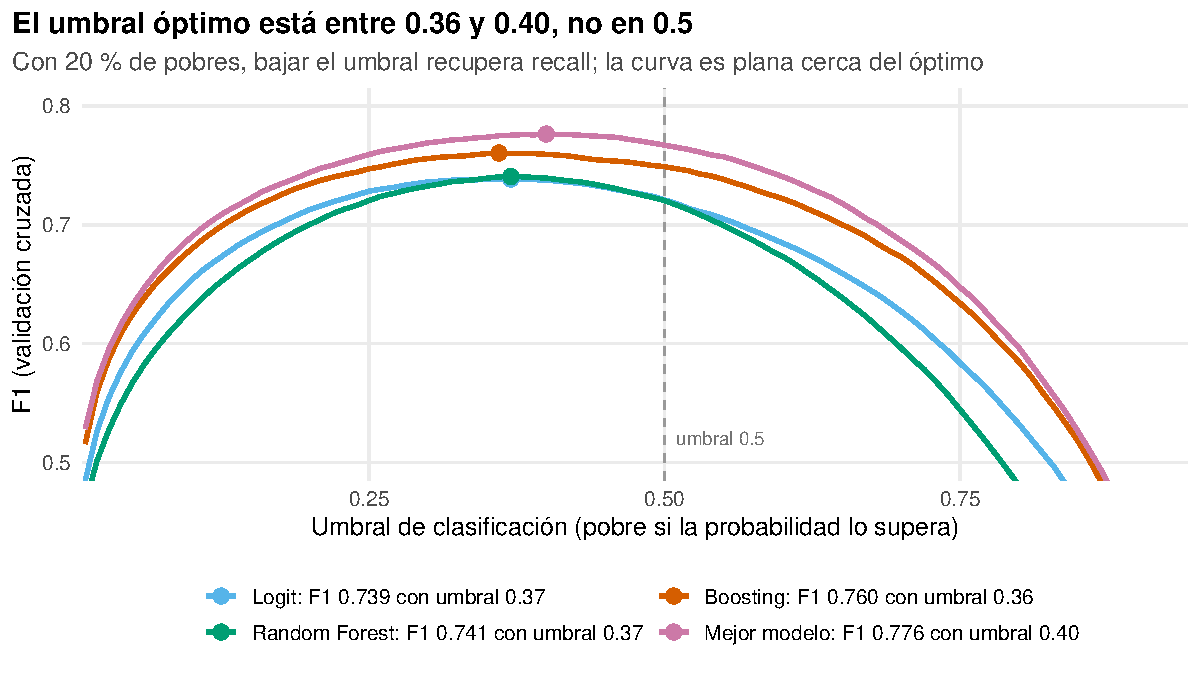
\includegraphics[height=0.47\textheight]{fig_curvas_umbral.pdf}
\par\vspace{0.3em}
\begin{columns}[c]
\begin{column}{0.6\textwidth}
\centering\tablar{\linewidth}{tab_desbalance}
\end{column}
\begin{column}{0.38\textwidth}
\footnotesize
\begin{itemize}
\item Bajar el umbral de 0.5 al óptimo sube el F1 entre 0.01 y 0.02 en todos los algoritmos.
\item Duplicar pobres (up-sampling) no agregó nada: solo cambió la escala de la probabilidad.
\end{itemize}
\end{column}
\end{columns}
\end{frame}

\begin{frame}{Del mejor algoritmo al mejor modelo: la información}
\centering
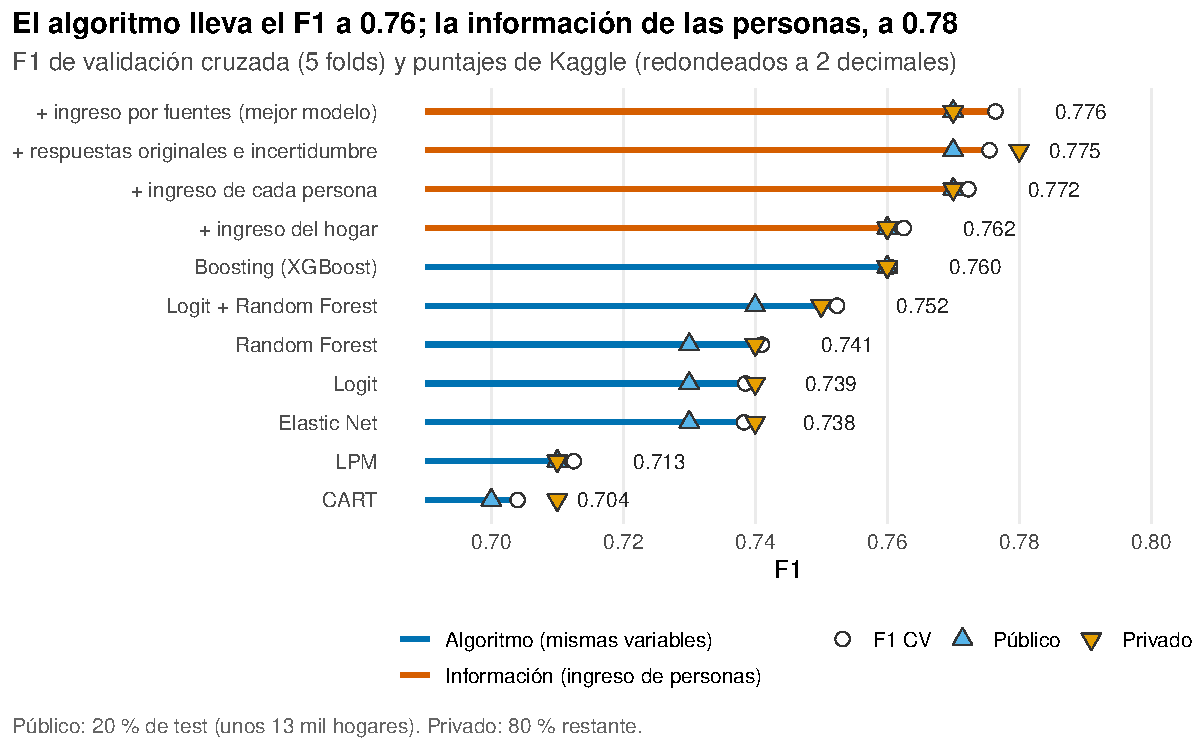
\includegraphics[height=0.86\textheight]{fig_escalera.pdf}
\end{frame}

\begin{frame}{Comparación detallada: el mejor frente a los dos que le siguen}
\centering
\vspace{0.4em}
\makebox[\linewidth]{\resizebox{1.07\linewidth}{!}{
\begin{threeparttable}
\begin{tabular}[t]{llcccccccc}
\toprule
Modelo & Qué cambia & F1 CV & Precisión & Recall & Dif. (EE) & Corr. & Cambian & Público & Privado\\
\midrule
\textbf{Mejor modelo} & \textbf{Clasificador + ingreso A, B y C} & \textbf{0.7764} & \textbf{0.748} & \textbf{0.806} & \textbf{---} & \textbf{1.000} & \textbf{---} & \textbf{0.77} & \textbf{0.77}\\
Ingreso A + B con sigma & Sin el ingreso por fuentes (C) & 0.7755 & 0.747 & 0.807 & -0.0009 (0.0006) & 0.999 & 0.7 \% & 0.77 & 0.78\\
LightGBM monótono + índice & LightGBM monótono (0.2) + índice (0.8) & 0.7762 & 0.754 & 0.800 & -0.0001 (0.0007) & 0.999 & 0.8 \% & 0.77 & 0.77\\
\bottomrule
\end{tabular}
\begin{tablenotes}
\item Mismos 5 grupos de validación. Dif. (EE): diferencia de F1 con el mejor, pareada por grupo, y su error estándar. Corr.: correlación de probabilidades con el mejor. Cambian: \% de hogares clasificados distinto que con el mejor.
\end{tablenotes}
\end{threeparttable}
}}
\par\vspace{1.2em}\raggedright
\small
\begin{itemize}\setlength\itemsep{0.6em}
\item \textbf{Empatados:} las diferencias de F1 (0.0009 y 0.0001) son \alert{menores que su error estándar}, sus probabilidades tienen correlación de 0.999 y clasifican distinto a menos del 1 \% de los hogares. El 0.78 privado de la versión A + B es ruido.
\item \textbf{Lección:} el ensamble con LightGBM monótono solo cambia el clasificador (\alert{14 restricciones de signo}) y empata: con el índice de ingreso adentro, \alert{el algoritmo del clasificador ya no importa}.
\end{itemize}
\end{frame}

\begin{frame}{La validación cruzada predijo a Kaggle}
\begin{columns}[c]
\begin{column}{0.7\textwidth}
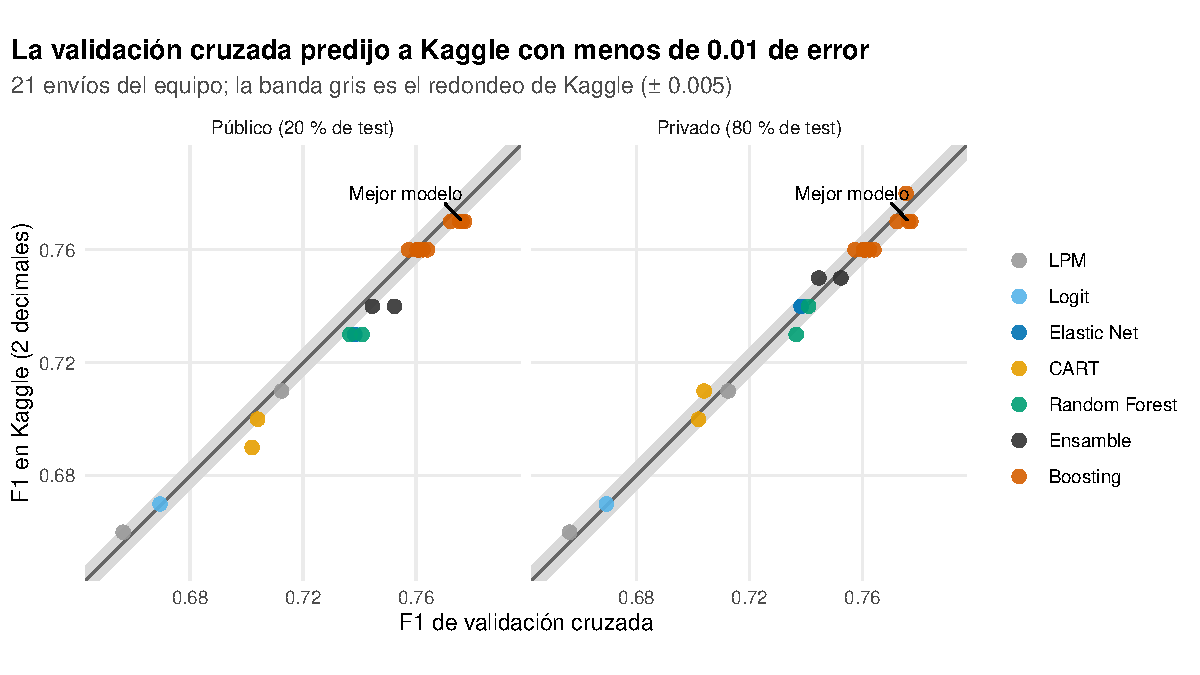
\includegraphics[width=\linewidth]{fig_cv_kaggle.pdf}
\end{column}
\begin{column}{0.29\textwidth}
\footnotesize
\begin{itemize}
\item Correlación CV--privado: \alert{0.99} en 21 envíos.
\item Decidimos con el CV, no con el público (ruido de $\pm 0.006$ con 13 mil hogares).
\item El ensamble con dos modelos de ingreso sacó 0.78 en el privado y el elegido (tres) 0.77, con CV de 0.7755 frente a 0.7764: es \alert{ruido}.
\end{itemize}
\end{column}
\end{columns}
\end{frame}

% ------------------------------------------------------------------------------
\section{Conclusión}

\begin{frame}{¿Qué modelo le recomendaríamos a una entidad del gobierno?}
\vspace{0.2em}
\makebox[\linewidth]{\resizebox{1.06\linewidth}{!}{
\begin{tabular}[t]{lcclll}
\toprule
Modelo & F1 CV & Privado & Interpretabilidad & Información & Entrenamiento\\
\midrule
Logit & 0.739 & 0.74 & Alta: coeficientes & Hogar (85 variables) & Minutos\\
Random Forest & 0.741 & 0.74 & Media: importancia & Hogar (85 variables) & 25 min por bosque\\
Boosting (XGBoost) & 0.760 & 0.76 & Media: importancia & Hogar (85 variables) & 1 min por ajuste\\
LightGBM con 10 variables & 0.689 & --- & Media: 10 variables & Hogar (10 variables) & 1 min\\
\textbf{Mejor modelo} & \textbf{0.776} & \textbf{0.77} & \textbf{Baja: 7 modelos encadenados} & \textbf{Hogar + ingresos de cada persona} & \textbf{2 horas}\\
\bottomrule
\end{tabular}
}}
\par\vspace{0.9em}
\begin{columns}[T]
\begin{column}{0.42\textwidth}
\footnotesize
\textbf{Complejidad frente a desempeño.} De logit a boosting: +0.02 sin perder variables. Del boosting al mejor modelo: +0.016, pero con nueve modelos de árboles y el módulo de ingresos.
\par\vspace{0.4em}
\textbf{Incentivos.} Si el puntaje decide el subsidio, los hogares aprenden a responder para obtenerlo.
\end{column}
\begin{column}{0.56\textwidth}
\begin{exampleblock}{Recomendación}
\small Para focalizar: \alert{boosting a nivel hogar} con preguntas verificables, restricciones de signo para que sea auditable y un umbral elegido por el costo de los errores. El mejor de Kaggle no es necesariamente el mejor instrumento.
\end{exampleblock}
\end{column}
\end{columns}
\end{frame}

\end{document}
